%!TEX program = xelatex
%!TEX root = ./thesis.tex
\section{Hierarchical Reinforcement Learning Methods}
%TODO: provide a informative overview on HRL methods

The paradigm of hierarchical reinforcement learning focuses on reducing the complexity of problems through temporal abstraction~\cite{barto2003recent}. A hierarchical reinforcement learning agent invokes temporally extended activities, which are low-level closed-loop partial policies instead of primary actions. Hierarchical reinforcement learning agents have two advantages: First, it does not need to make a decision at every time step and thus the time scale is reduced. Second, it could reuse the existing temporally extended activities and thus the learning efficiency might be improved if they are useful in many cases.

The study of hierarchical reinforcement learning has a long history of around 20 years~\cite{sutton1999between}. Many methods have been proposed,  and some of the representative works include option framework~\cite{sutton1999between}, hierarchies of abstract machines~\cite{parr1998reinforcement}, and MAXQ value function decomposition~\cite{dietterich2000hierarchical}.

All the hierarchical reinforcement learning methods need to solve 2 problems. The first problem is to define and learn the low-level partial policies. Second is to learn the selection and scheduling of the low-level partial policies, including the selection of the partial policies and the scheduling of the decision points.

The first problem has been studied from different point of views. The ideal problem formulation is that the agent should directly discover the useful low-level partial policies. However, the solution for general cases in this formulation infeasible although methods have been proposed~\cite{mcgovern2001automatic},~\cite{hengst2002discovering} for some special cases. 

The most practical formulation is to manually define the low-level partial policies as well as the scheduling criteria of them. However, it heavily relies on domain-specific engineering, and manually defining a set of predefined low-level partial policies with their scheduling criteria might not be possible. Another popular formulation is to propose a set of auxiliary MDPs to define and train the low-level policies. The partial-policies will also be terminated if the current auxiliary MDP has terminated in the target environment. However, this formulation is also limited to the special cases of goal-directed environments with a finite set of possible goals. 

The formulation of this thesis is the low-level policies are defined trained in a set of given source tasks. The problem of selecting and scheduling them is left to be solved. This formulation can handle many general cases and the target problem can be solved as long as it can be decomposed into a series of source tasks. The formulation may not be feasible for some complex problems like the board game GO. But a vast majority of real-world problems could be decomposed by a series of simple primary tasks. For example, the task of navigating a robot to a target location can be decomposed into the tasks of moving forward, turning left/right, going downstairs/upstairs, bypassing an obstacle and opening/closing a door. The task of assembling a hardware product can be decomposed into combining two specific components, plugging in the wires, installing the screws and etc.

The solution of learning to select among low-level policies, has been thoroughly studied by the Semi-Markov Decision Process (SMDP) theory since the work of~\cite{sutton1999between}. However, a general solution to the scheduling of the partial policies is still missing.

The following sections will discuss the related works of hierarchical reinforcement learning methods in details.

\subsection{Option Framework}
The option framework \cite{sutton1999between} is one of the earliest studies in hierarchical reinforcement learning. The author uses the notion of \textit{option} to define the partial policies. A complete definition of option consists of an input set $I$, a partial policy $\pi$ and a termination condition $\beta$. The input set $I$ is a set of states where the option is permitted to be executed. The partial policy $\pi$ is a mapping form the input set to the action space, which defines the policy to be executed during the activation period of the option. The termination condition $\beta$ is a mapping from the current state-action pair to a scalar value that controls when the option should be terminated.

An option is Markov if its policy is Markov. Semi-Markov options, on the other hand, are options whose policies not only take the current state as input, but also are based on the state history since initiation of the current option. A policy over options \(\mu \) selects option \(o\) in state \(s\) with probability \(\mu(s,o)\). 
%The concept of multi-step model is proposed as a generalization of single-step models. 
For any option \(o\), let \(E(o,s,t)\) denote the event of the option $o$ initialized in state $s$ at time $t$. The return of the multi-step model is defined as:
\[ R(s,o)=E\{r_{t+1}+\gamma r_{t+2}+\ldots+\gamma^{t+\tau} r_{t+\tau} \lvert E(o,s,t\} \]
where $t+\tau$ is the termination time of $o$. The state transition model for the option is:
\[P(s' \lvert s,o)=\sum_{\tau=1}^{\infty} p(s',\tau) \gamma^\tau \]
for all states \(s' \in S \), where \( p(s',\tau) \) denotes the probability that the option terminates after \(\tau\) steps and results in the state \(s'\).

A generalized form of the Bellman optimality equation is then proposed:
\begin{equation}
    V_O^*(s) = \max_{o \in O_s} \big[ R(s,o)+\sum_{s'}P(s' \lvert s,o) V_O^*(s') \big]
\end{equation}
% The optimal policies over options are in general suboptimal policies in the original MDP when some of the primitive actions are not available as 1-step options.
The option framework proposes a formulation of hierarchical reinforcement learning and connects it to SMDP theory. The authors also propose the method for training the policy over options. However, the question on how the hierarchy of options is developed is not answered.

\subsection{Modulated Hierarchical Controller}
The study of \cite{heess2016learning} applies hierarchical reinforcement learning in deep reinforcement learning for continuous control problems. They propose a two-level hierarchical agent architecture consisting of a high-level (HL) policy and a low-level (LL) policy. The high-level policy produces a modulation signal which the low-level agent then takes as part of its input. The architecture is demonstrated in Figure~\ref{review_moduler_arch}.
\begin{figure}[h]
	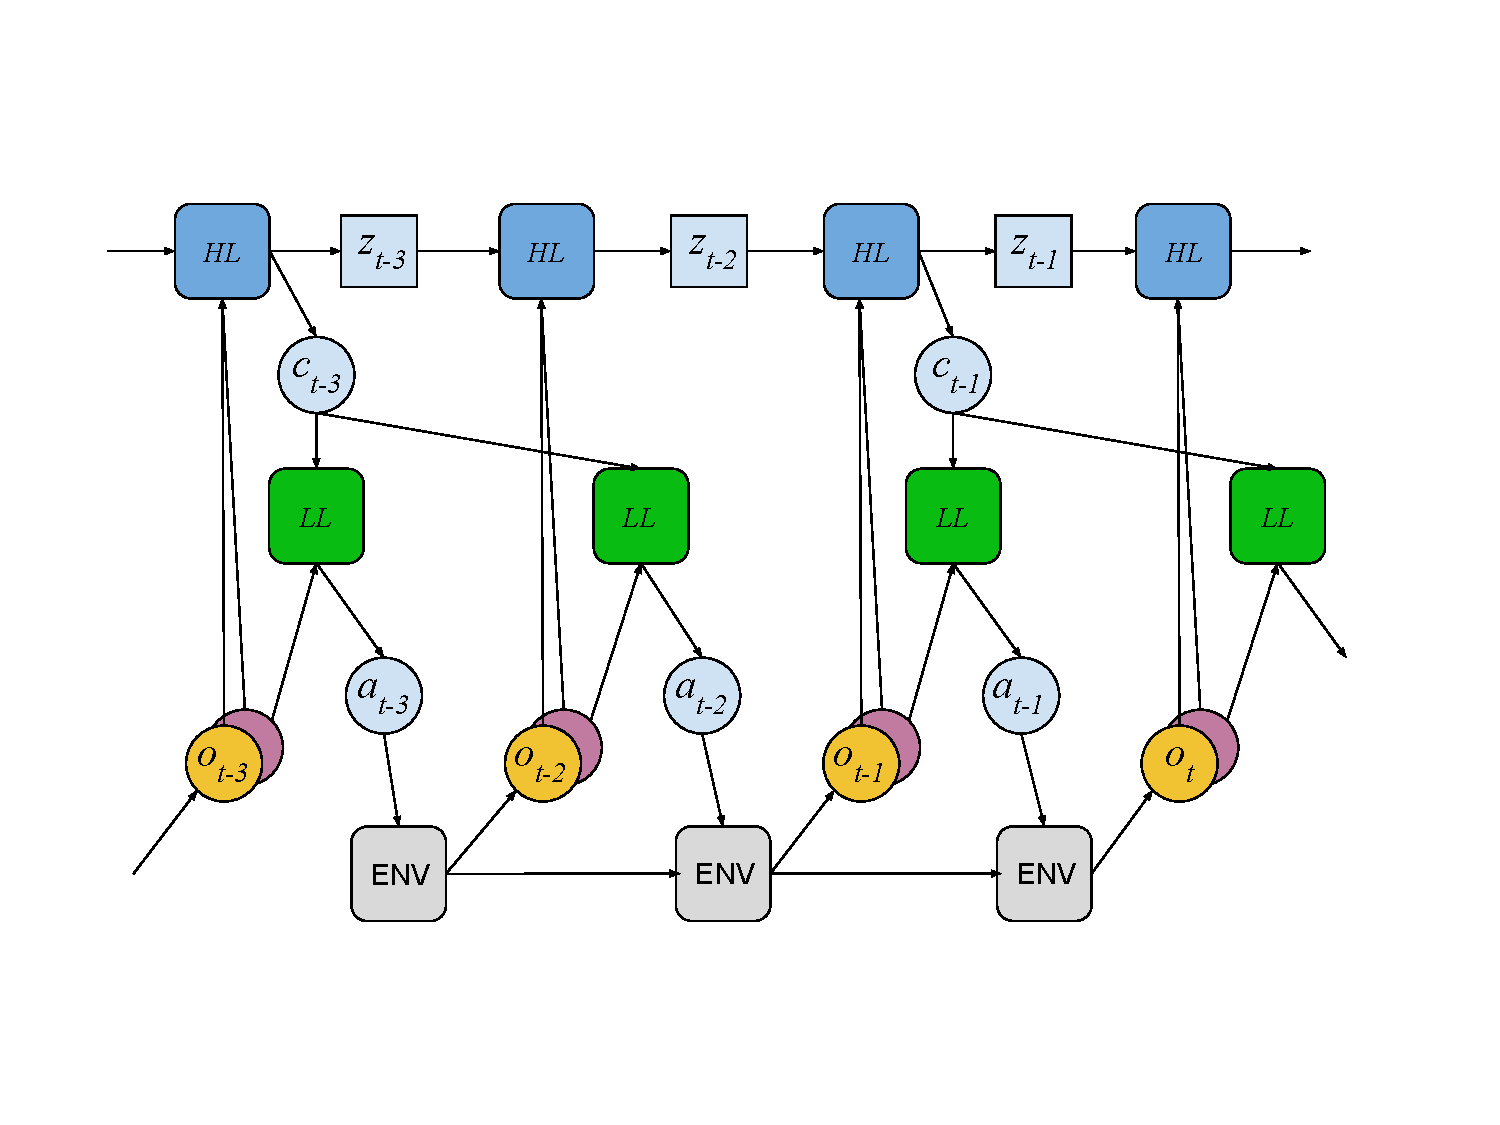
\includegraphics[width=\textwidth]{review_moduler_arch.pdf}
	\centering
	\caption{The hierarchical structure of the modulated controller~\cite{heess2016learning}, which consists
		of the recurrent high-level controller (HL, dark blue) and
		feedforward low-level controller (LL, green).  The
		high-level controller has access to all observations (yellow and red). While both controllers observe sensory
		input at the world-clock frequency, the modulatory control signal from the high-level is updated every K
		steps (here K = 2)}\label{review_moduler_arch}
\end{figure}
The hierarchical agent is characterized by a policy $\pi$ with parameter $\theta$. The policy is defined by the composition of the high-level controller $F_H$ and low-level controller $F_L$. The low-level controller is a feed-forward neural network that maps the preprocessed current state $o(s)$ and the control signal from the high-level controller $c$ to the policy output.
\begin{align}
\pi (a| s) = F_L(o(s),c)
\end{align}
where the preprocessed state $o(s)$ removes task-specific information from the current state.
The high-level controller is a recurrent neural network: $F_H = (f_z,f_c)$ that produces the new control signal at every $K$ time step:
\begin{align}
z_t = f_z(s_t,z_{t-1}) \\
c_t = f_c(z_{t_r})
\end{align}
where $t_r$ is the most recent update output of the control signal. A predefined Gaussian noise component is added to the output $c_t$ during the training of the high-level controller, so that the agent has a better performance in exploration.
The training of the hierarchical agent consists of two separate phases: pre-training and transfer. The tasks used for pre-training are relatively simple tasks that facilitate the development of generic locomotion skills. After pre-training, the high-level controller is re-initialized and the weights of low-level controllers are frozen. The high-level controller is then trained in the transfer task, which has a sparse reward function.

This method manages to solve a few problems with sparse reward functions and low-dimensional state inputs that can not be solved by any flat reinforcement learning methods. The limitation is that the architecture requires heavy problem-specific engineering efforts. The observation of the low-level agent $o(s)$ is designed manually. The hierarchical relationships between the two agents, including the definition of pre-training environments and the modulation architecture, are also predefined. Apart from that, the low-level agent can only be executed for a fixed number ($K$) of time-steps before it gets terminated. As a result, this design could only be useful in a limited class of problems.

\subsection{Hierarchical Reinforcement Learning by Meta-learning}
Another work~\cite{frans2017meta}, namely meta learning shared hierarchies (MLSH), proposes a meta-learning approach for learning hierarchically structured policies.
The MLSH method formulates the problem as learning a finite set of MDPs $P_M$ with the same state-action space, using a universal agent architecture. The agent consists of two sets of parameters $(\phi,\theta)$, where $\phi$ is the set of task-independent parameters and $\theta$ is the set of task-specific parameters. The meta-learning objective is to optimize the expected return during the agent's entire lifetime:
\begin{align}
\mathrm{maximize}_\phi \mathbb{E}_{M\sim P_M}[R]
\end{align}
The detailed structure of the agent is shown in Figure~\ref{review_mlsh_arch}. The architecture is a two-level hierarchical reinforcement learning agent, the components $\phi_1,\phi_2,\dots$ are the parameters of the low-level agent policies (called sub-policies) and are shared across different tasks. $\theta$ is the parameters of the high-level agent of the current task. The policy of the high-level agent, namely master policy, samples an action at fixed periods and selects the sub-policy to be executed.
\begin{figure}[h]
	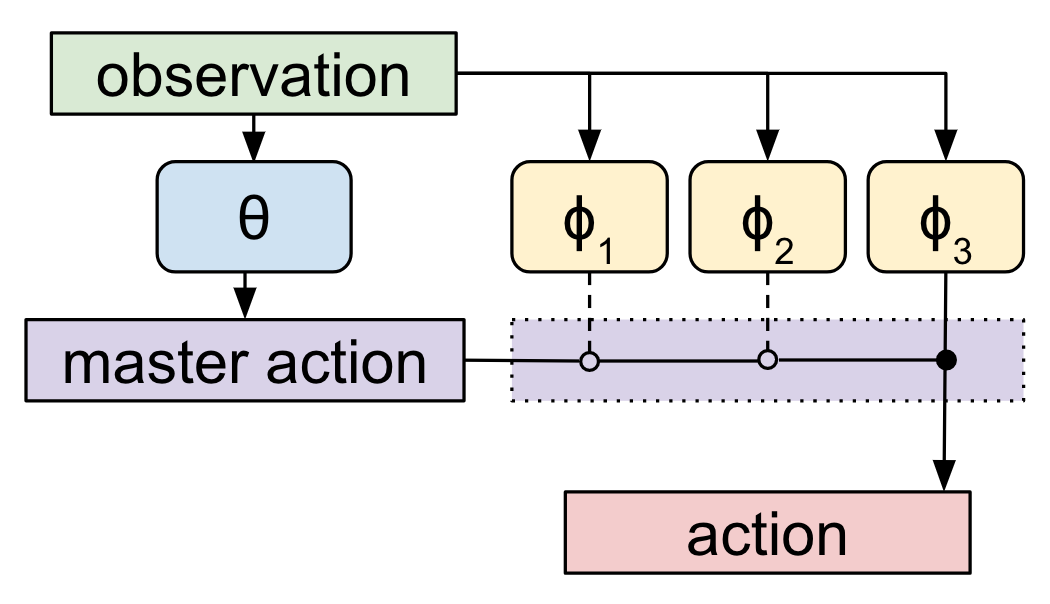
\includegraphics[width=0.5\textwidth]{review_mlsh_setup.png}
	\centering
	\caption{The agent setup of the modulated controller~\cite{frans2017meta},$\theta$ represents the master policy, which selects
		a sub-policy to be active. In the diagram, $\phi_3$ is the active sub-policy, and actions are taken according
		to its output.}\label{review_mlsh_arch}
\end{figure}
The agent is trained in the following manner: First a task is sampled $M$ is sampled and the parameter $\theta$ is re-initialized randomly. Then there is a warmup phase, where only $\theta$ is trained to be optimal. Then the agent enters the joint update phase, where both $\theta$ and $\phi$ are updated simultaneously.
The method achieves good performance in several control environments. Including a moving-bandit Ant-robot task, an Ant robot maze navigation task and an obstacle course task. 

However, the tasks are actually simplified versions of the control tasks defined in \cite{duan2016benchmarking}. One modification is that the state of the Ant robot is periodically reset to prevent episode termination due to the falling of the robot. The complexity of the control task is thus largely reduced. It is not clear whether the method would perform well on the original version of the Ant environment.
The MLSH method also relies on a warm-up period to learn the high-level agent's policy. However, the authors didn't provide a solution to learn the high-level agent's policy $\theta$ at the beginning where the parameter $\phi$ is also randomly initialized.
Finally also predefines the temporal relationship between the high-level policy and low-level policy, and the master agent only makes decisions at fixed periods.
% \section{Hindsight Experience Replay}
% The work of~\cite{andrychowicz2017hindsight} generate actuator policies and there corresponding termination predicate policies based on the definition of subgoals. The subgoals are generated by heuristic functions of a target state. TODO
% \section{Scheduled Auxiliary Control}
% The work of \cite{riedmiller2018learning} proposes the method of scheduled auxiliary control. The method generates partial policy by a given set of simple auxiliary tasks, whose reward signals are generated based on heuristic functions of the sensor activation. The method also assume a constant execution length of the actuator policies. TODO
\subsection{Goal-directed Learning Methods}
Several works~\cite{riedmiller2018learning}, ~\cite{andrychowicz2017hindsight} have attempted to solve sparse-reward robot control environments through the learning of auxiliary MDPs.
The method of~\cite{riedmiller2018learning}, namely Scheduled Auxiliary Control (SAC-X), is one of the representative works and is based on several main principles. First, the original MDP is modified, where the agent receives a vector reward signal at each timestep, consisting of the reward for the original MDP and a set of internal auxiliary rewards. Second, each internal auxiliary reward function is assigned a low-level agent policy, namely intention. Third, there is a high-level agent that selects and executes the intentions. Fourth, the learning of intentions is performed off-policy on the same experience and is performed simultaneously for different intentions.
The definitions of internal auxiliary rewards are based on predefined goal states. The internal auxiliary reward with goal state $g$ is defined as:
\begin{equation}
r_g(s,a)=
\begin{cases}
\delta_g(s),& \text{if } d(s,g)\\
0,              & \text{else}
\end{cases}
\end{equation}
The parameter $\theta$ of the intentions is trained with the aggregation of loss of all the reward functions:
\begin{align}
\mathcal{L}(\theta)  = \mathcal{L}(\theta;M) +\sum_{k=1}^{|A|} (\mathcal{\theta;A_K})
\end{align}
Where $M$ is the MDP with the original reward function and $A=\{A_1,\dots,A_k\}$ is the set of MDPs with internal auxiliary rewards. The training of the intention parameter is formulated as a multi-task RL problem.
The high-level scheduler policy is the trained using an off-policy policy gradient method with $\theta$ being fixed.
The method manages to solve the object grasping and stacking problems in a robot-arm environment. 

One limitation of SAC-X is that the method relies on predefined auxiliary MDPs. Proposing auxiliary MDPs could be solved by using heuristic algorithms, but such heuristic algorithms are only available for some special problems. Apart from that, the method limits the definition of auxiliary MDPs to be goal-directed tasks, which is impractical for the more realistic high-dimensional state-space problems.


\subsection{Other Methods Targeting at Environments with Sparse Reward Function}
Apart from the above-mentioned works, several other methods have also been proposed to solve environments with sparse reward recently, including Unicorn~\cite{mankowitz2018unicorn}, FuN~\cite{vezhnevets2017feudal},  HRL with Stochastic Temporal Grammar~\cite{shu2017hierarchical}, policy sketch method~\cite{andreas2016modular} and strategic attentive writer~\cite{vezhnevets2016strategic}. These methods are only verified in discrete environments and no evidence has shown that they are applicable to our target problem domains.